\documentclass{article}
\usepackage{polski}
\usepackage[utf8]{inputenc}
\usepackage[pdftex,dvips]{graphicx}
\usepackage{hyperref}

\graphicspath{ {img/} }

\author{Rafał Lisiecki}
\title{Liczby pierwsze i złożone}
\begin{document}

\maketitle


\newpage

\newtheorem{example}{Przykład}
\newtheorem{diagram}{Diagram}
\newtheorem{krok}{Krok}
\newtheorem{twierdzenie}{Twierdzenie}

\tableofcontents

\newpage
\section{Wstęp}
\begin{center}
\textit{
,,Zagadnienie odróżniania liczb pierwszych od złożonych i rozkładanie tych ostatnich na czynniki pierwsze uchodzi za najważniejsze i o dużym praktycznym znaczeniu w arytmetyce. ''}
\end{center}
\begin{flushright} \texttt{Carl Friedrich Gauss} \end{flushright}


Iloczyn liczb naturalnych jest zawsze liczbą naturalną, są więc liczby naturalne, będące iloczynami dwóch liczb naturalnych większych od jedności. Są także liczby naturalne większe od jedności, które nie są iloczynami dwóch liczb naturalnych większych od jedności. Takie właśnie liczby nazywamy pierwszymi. Liczby pierwsze to swego rodzaju cegiełki służące do budowania kolejnych liczb naturalnych.
\\
Liczby pierwsze to liczby naturalne, które posiadają dokładnie dwa dzielniki (liczbę 1 i samą siebie).

\begin{example} Kilka początkowych liczb pierwszych: 2,3,5,7,11,13,17,19, \ldots \end{example}

Jeśli liczba naturalna większa od 1 nie jest liczbą pierwszą, to jest iloczynem dwóch liczb naturalnych od niej mniejszych. Liczby takie nazywamy liczbami złożonymi.

Liczby złożone to liczby naturalne, które posiadają więcej niż dwa dzielniki.

\begin{example} Kilka początkowych liczb złożonych: 4,6,8,9,10,12,14,15, \ldots \end{example}

Liczby 0 i 1 nie należą ani do liczb pierwszych ani do złożonych. Kiedyś uznawano liczbę 1 za pierwszą, jest ona jednak tak różna od właściwych liczb pierwszych, że dziś lokuje się ją w odrębnej klasie, nosi nazwę jedności.

\newpage

\section{Rozpoznawanie liczby pierwszej}

\subsection{Szukanie dzielników liczby}
Aby sprawdzić, czy liczba naturalna jest liczbą pierwszą, należy dzielić ją kolejno przez wszystkie liczby większe od 1 i mniejsze równe pierwiastka kwadratowego z tej liczby. Jeśli przy każdym dzieleniu reszta z dzielenia jest różna od zera, to liczba jest liczbą pierwszą. Natomiast jeżeli choć jedno dzielenie daje resztę równą zero, to sprawdzana liczba naturalna jest liczbą złożoną. Nie jest to więc problem teoretyczny, jednak praktycznie trudny w przypadku bardzo dużych liczb.

\begin{diagram}
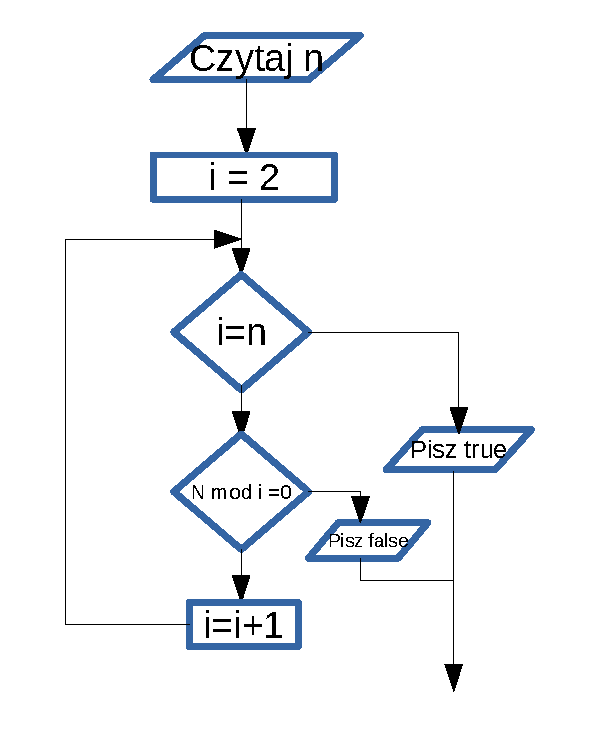
\includegraphics{1.pdf}
\end{diagram}


Jeśli liczba jest stosunkowo niewielka, takie dzielenia możemy przeprowadzić sami, natomiast jeśli liczba nie jest już mała, to można ją sprawdzić z pomocą komputera. Maszynę trzeba zaprogramować, czyli napisać algorytm, który rozstrzygnie, czy dana liczba jest pierwsza. Algorytm ten musi być przy tym efektywny, taki, który wykona możliwie jak najmniej operacji.

\subsection{Sito Eratostenesa}

Problemem liczb pierwszych zajmowali się matematycy od bardzo dawna. Jednym z nich był matematyk grecki Eratostenes z Cyreny, żyjący w III w. p.n.e. Wymyślona przez niego metoda wyznaczania wszystkich liczb pierwszych nie większych od zadanej liczby nosi do dziś nazwę sita Eratostenesa.

Aby sprawdzić, czy liczba naturalna \textit{n} jest liczbą pierwszą, należy dzielić ją przez każdą taką liczbę \(k>1 \), gdzie \(k^{2}\leq n\). Sposób ten nie jest najbardziej efektywną metodą, ponieważ trzeba wykonać dużą liczbę czasochłonnych dzieleń, tym większą, im większą wartość ma badana liczba.

Skoro łatwiej jest mnożyć niż dzielić, Eratostenes zamiast sprawdzać podzielność kolejnych liczb naturalnych, zaproponował usuwanie ze zbioru liczb naturalnych wielokrotności kolejnych liczb, które nie zostały wcześniej usunięte.

Sprawdźmy na przykładzie. Niech n=100.
Należy postępować następująco: wypisać wszystkie liczby do 100, wykreślić wszystkie wielokrotności liczby pierwszej 2, w każdym następnym kroku należy wykreślić wszystkie wielokrotności najmniejszej kolejnej nie wykreślonej liczby p, które są większe od p. Wystarczy to zrobić dla takich p, że \(p^{2}\leq 100\), w naszym przypadku dla liczb pierwszych 2,3,5,7. Wszystkie wielokrotności liczb 2,3,5,7 należy odsiać, liczby, które nie zostały wykreślone są liczbami pierwszymi.\cite{math}

\begin{krok} 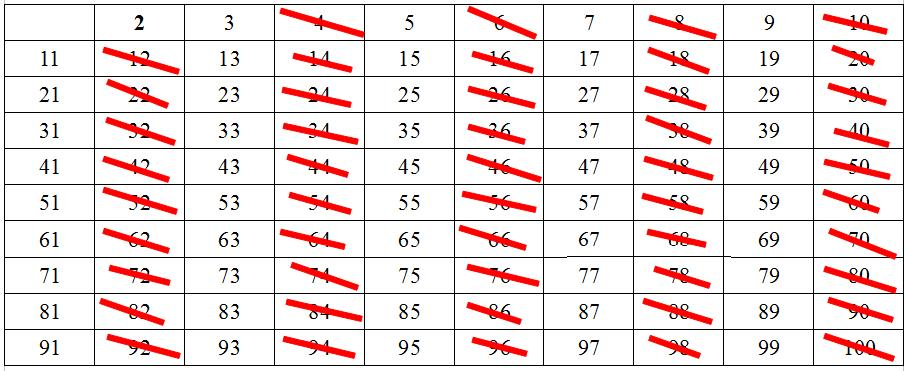
\includegraphics[scale=0.4]{2.jpg} \end{krok}
\begin{krok} 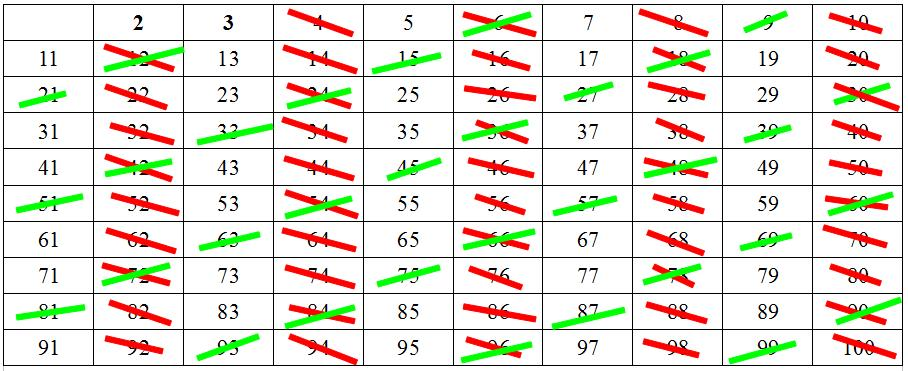
\includegraphics[scale=0.4]{3.jpg} \end{krok}
\begin{krok} 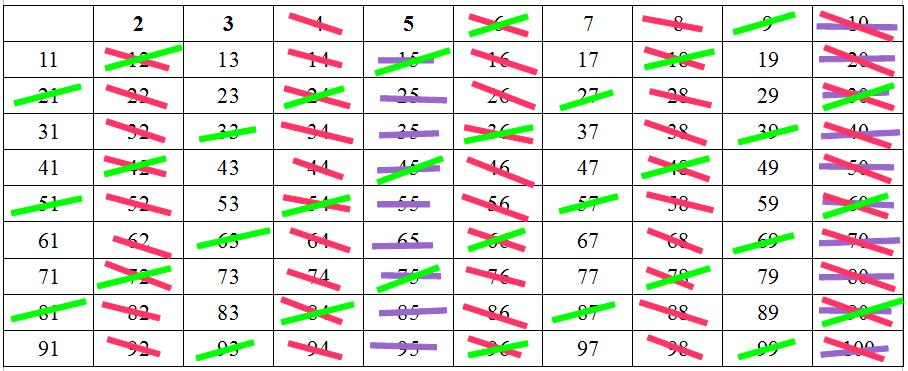
\includegraphics[scale=0.4]{4.jpg} \end{krok}
\begin{krok} 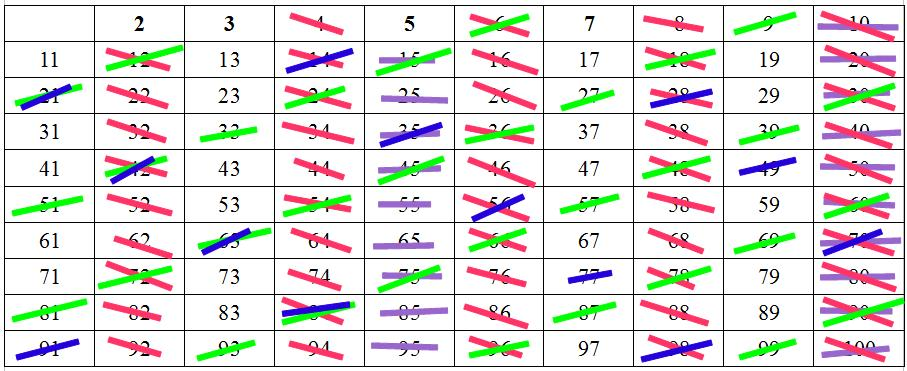
\includegraphics[scale=0.4]{5.jpg} \end{krok}
\begin{krok} 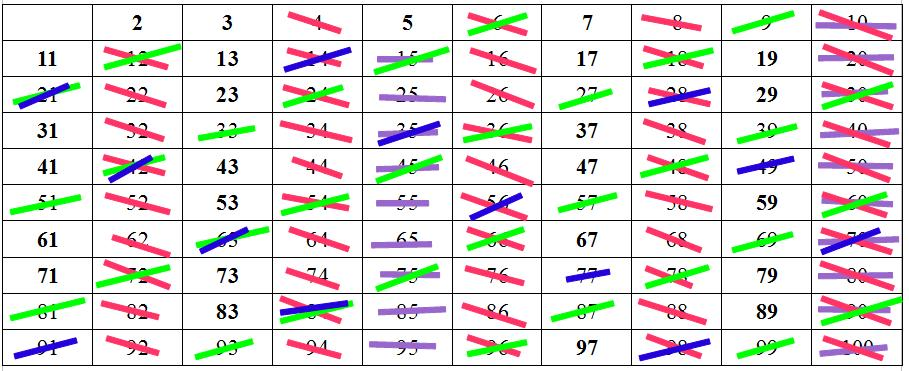
\includegraphics[scale=0.4]{6.jpg} \end{krok}

$$\left[\begin{array}{cccccccccc}
2&3&5&7&11&13&17&19&23&29\\
31&37&41&43&47&53&59&61&67&71\\
73&79&83&89&97&101&103&107&109&113\\
127&131&137&139&149&151&157&163&167&173\\
179&181&191&193&197&199&211&223&227&229
\end{array}\right]$$
W powyższej macierzy prezentuję liczby pierwsze takie że \( 1\leq p < 230 \)

\subsection{Twierdzenie Legrange'a}

\begin{twierdzenie}
Jeżeli p jest liczbą pierwszą, wielomian \(f(x)=a_{0}*x^{n}+a_{1}*x^{n-1}+\ldots+a_{n-1}*x+a_{n}\) jest wielomianem stopnia n o współczynnikach całkowitych, gdzie współczynnik a0 jest niepodzielny przez p, to wśród liczb \(x=0,1,2,\ldots,p-1\) istnieje nie więcej niż n takich, dla których liczba f(x) jest podzielna przez p.\cite{wiki}
\end{twierdzenie}

Wniosek z twierdzenia Lagrange'a:
Jeżeli p jest liczbą pierwszą, a f(x) jest wielomianem stopnia n o współczynnikach całkowitych, oraz jeżeli istnieje więcej niż n liczb naturalnych x<p, dla których f(x) jest podzielne przez p, to wszystkie współczynniki wielomianu f(x) muszą być podzielne przez p.

\subsection{Funkcja L. Eulera}
L. Euler, poszukując różnowartościowej funkcji przporządkowującej liczbom naturalnym liczby pierwsze, zwrócił uwagę na funkcję f: \( N \to N \) taką, że: \\
\begin{center} \(f(n) = n^{2} + n + 41 \) \cite{topp}
\newline \newline \newline

\begin{tabular}{|c|c|}
  \hline 
  X & \(f(x) = x^{2} + x + 41 \)\\
  \hline
  0 & 41 \\
  \hline
  1 & 43 \\
  \hline
  2 & 47 \\
  \hline
  3 & 53 \\
  \hline
  4 & 61 \\
  \hline
  5 & 71 \\
  \hline
  6 & 83 \\
  \hline
  7 & 97 \\
  \hline
  8 & 113 \\
  \hline
  9 & 131 \\
  \hline
  10 & 151 \\
  \hline
\end{tabular}  \end{center}
W powyżej tabeli prezentuje wartości funkcji\( f(n)\) dla \(x\) takich że: \( 0 < x \leq 10\)

\newpage
\begin{thebibliography}{9}
\bibitem{topp}
  Jerzy Topp,
  \emph{Wstęp do MATEMATYKI}.
  Gdańsk:
  Wydawnictwo Politechniki Gdańskiej
  2012
\bibitem{wiki}
  Wikipedia,
  \emph{\url{http://pl.wikipedia.org/wiki/Liczba_pierwsza}}.

\bibitem{math}
 Math.edu.pl,
\emph{\url{http://www.math.edu.pl/liczby-pierwsze}}

\end{thebibliography}
\end{document}
